\documentclass[11pt]{article}
\usepackage{fullpage}
\usepackage{algorithm}
\usepackage[noend]{algorithmic}
\usepackage{enumerate}
\usepackage{amsmath,amssymb,amsthm}
\usepackage{stackrel}
\usepackage{tikz}

% Helpful Shortcuts
\newcommand{\bc}[1]{{\quad \text{(#1)}}} 	% Justification in math env
\newcommand{\st}{{\text{ such that }}} 							   % Math env
\newcommand{\abs}[1]{{ |#1 |}} 							% Absolute value / Cardinality
\newcommand{\bld}[2]{\noindent\textbf{#1:}\hspace{0.1in}#2$  $\bigskip} % Headings
\newcommand{\notimplies}{%
	\mathrel{{\ooalign{\hidewidth$\not\phantom{=}$\hidewidth\cr$\implies$}}}}
\newcommand{\linesep}{\noindent\bigskip\rule{17cm}{0.1mm}\bigskip} % Horizontal Line

% These define new environments / formats for lemmas, definitions, running time, etc.
\newtheorem{lemma}{Lemma}
\newtheorem{definition}{Definition}
\newtheorem{notation}{Notation}
\newtheorem*{claim}{Claim}
\newtheorem{observation}{Observation}
\newtheorem{conjecture}[lemma]{Conjecture}
\newtheorem{theorem}[lemma]{Theorem}
\newtheorem{corollary}[lemma]{Corollary}
\newtheorem{proposition}[lemma]{Proposition}
\newtheorem*{rt}{Running Time}

% These define nice ways to format P and OPT (use \P or \opt)
\def\P{\ensuremath{$ \mathcal{P} $}}
\def\opt{\ensuremath{\textsc{opt}}}
\renewcommand{\labelenumi}{\bf \alph{enumi}.}

\renewcommand\maketitle{
	\begin{center}
		\begin{tabular*}{6.44in}{l @{\extracolsep{\fill}}c r}
			\bfseries  &  & \bfseries CSCI 383 Spring 2019 \\
			\bfseries&  & \bfseries  Homework \#5 Solutions  \\
			\bfseries   &   &  \bfseries Kai Ting Keshia Yap\\ 
		\end{tabular*}
\end{center} }

\begin{document}
	\maketitle
	\noindent Honor Code: I affirm that I adhered to the Honor Code in this assignment. Keshia Yap\\
	\subsection*{Part  3: Regex Against the Machines}
	\begin{enumerate} [1.]
	\item $ (0 + 1)^*000(0 + 1)^* $: The regular expression $ A:=(0 + 1)^* $ refers to any string in the language $ \{0,1\} $. So the entire regular expression is $ A000A $ which denotes the language that accepts any string with at least three consecutive 0's.
	\begin{center}
		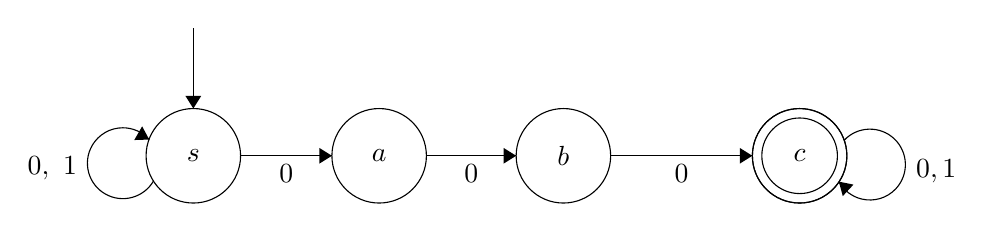
\begin{tikzpicture}[scale=0.2]
		\tikzstyle{every node}+=[inner sep=0pt]
		\draw [black] (21.2,-25.1) circle (3);
		\draw (21.2,-25.1) node {$s$};
		\draw [black] (33,-25.1) circle (3);
		\draw (33,-25.1) node {$a$};
		\draw [black] (44.7,-25.1) circle (3);
		\draw (44.7,-25.1) node {$b$};
		\draw [black] (59.7,-25.1) circle (3);
		\draw (59.7,-25.1) node {$c$};
		\draw [black] (59.7,-25.1) circle (2.4);
		\draw [black] (59.7,-25.1) circle (3);
		\draw [black] (24.2,-25.1) -- (30,-25.1);
		\fill [black] (30,-25.1) -- (29.2,-24.6) -- (29.2,-25.6);
		\draw (27.1,-25.6) node [below] {$0$};
		\draw [black] (36,-25.1) -- (41.7,-25.1);
		\fill [black] (41.7,-25.1) -- (40.9,-24.6) -- (40.9,-25.6);
		\draw (38.85,-25.6) node [below] {$0$};
		\draw [black] (47.7,-25.1) -- (56.7,-25.1);
		\fill [black] (56.7,-25.1) -- (55.9,-24.6) -- (55.9,-25.6);
		\draw (52.2,-25.6) node [below] {$0$};
		\draw [black] (62.523,-24.12) arc (136.87498:-151.12502:2.25);
		\draw (67.07,-26.07) node [right] {$0,1$};
		\fill [black] (62.19,-26.74) -- (62.44,-27.66) -- (63.12,-26.93);
		\draw [black] (18.673,-26.696) arc (-29.99099:-317.99099:2.25);
		\draw (13.84,-25.9) node [left] {$0,\mbox{ }1$};
		\fill [black] (18.4,-24.07) -- (17.95,-23.23) -- (17.45,-24.1);
		\draw [black] (21.2,-17) -- (21.2,-22.1);
		\fill [black] (21.2,-22.1) -- (21.7,-21.3) -- (20.7,-21.3);
		\end{tikzpicture}
	\end{center}

	\item $ (((00)^*(11)) + 01)^* $: Accepts the concatenation of any number of copies of $ 01 $ and $ (00)^*11 $. I first built NFAs for 00, 11 and 01, and added epsilon transitions to concatenate/union/asterate them, and then simplified the NFA by removing the epsilon transitions.
	
	
	\begin{center}
		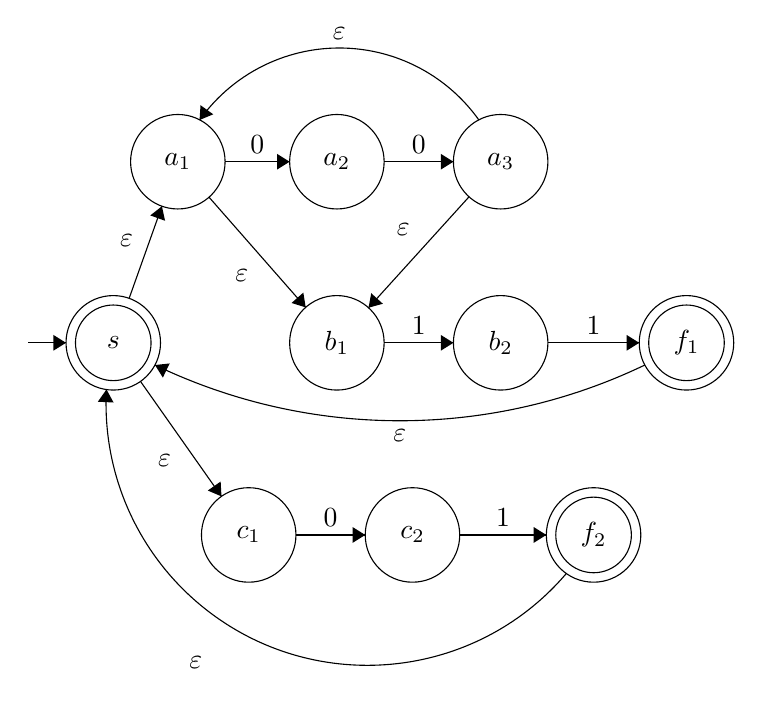
\begin{tikzpicture}[scale=0.2]
		\tikzstyle{every node}+=[inner sep=0pt]
		\draw [black] (10.5,-21.4) circle (3);
		\draw (10.5,-21.4) node {$a_1$};
		\draw [black] (20.6,-21.4) circle (3);
		\draw (20.6,-21.4) node {$a_2$};
		\draw [black] (31,-21.4) circle (3);
		\draw (31,-21.4) node {$a_3$};
		\draw [black] (20.6,-32.9) circle (3);
		\draw (20.6,-32.9) node {$b_1$};
		\draw [black] (31,-32.9) circle (3);
		\draw (31,-32.9) node {$b_2$};
		\draw [black] (42.8,-32.9) circle (3);
		\draw (42.8,-32.9) node {$f_1$};
		\draw [black] (42.8,-32.9) circle (2.4);
		\draw [black] (15,-45.1) circle (3);
		\draw (15,-45.1) node {$c_1$};
		\draw [black] (25.4,-45.1) circle (3);
		\draw (25.4,-45.1) node {$c_2$};
		\draw [black] (36.9,-45.1) circle (3);
		\draw (36.9,-45.1) node {$f_2$};
		\draw [black] (36.9,-45.1) circle (2.4);
		\draw [black] (6.4,-32.9) circle (3);
		\draw (6.4,-32.9) node {$s$};
		\draw [black] (6.4,-32.9) circle (2.4);
		\draw [black] (13.5,-21.4) -- (17.6,-21.4);
		\fill [black] (17.6,-21.4) -- (16.8,-20.9) -- (16.8,-21.9);
		\draw (15.55,-20.9) node [above] {$0$};
		\draw [black] (23.6,-21.4) -- (28,-21.4);
		\fill [black] (28,-21.4) -- (27.2,-20.9) -- (27.2,-21.9);
		\draw (25.8,-20.9) node [above] {$0$};
		\draw [black] (23.6,-32.9) -- (28,-32.9);
		\fill [black] (28,-32.9) -- (27.2,-32.4) -- (27.2,-33.4);
		\draw (25.8,-32.4) node [above] {$1$};
		\draw [black] (34,-32.9) -- (39.8,-32.9);
		\fill [black] (39.8,-32.9) -- (39,-32.4) -- (39,-33.4);
		\draw (36.9,-32.4) node [above] {$1$};
		\draw [black] (18,-45.1) -- (22.4,-45.1);
		\fill [black] (22.4,-45.1) -- (21.6,-44.6) -- (21.6,-45.6);
		\draw (20.2,-44.6) node [above] {$0$};
		\draw [black] (28.4,-45.1) -- (33.9,-45.1);
		\fill [black] (33.9,-45.1) -- (33.1,-44.6) -- (33.1,-45.6);
		\draw (31.15,-44.6) node [above] {$1$};
		\draw [black] (28.99,-23.63) -- (22.61,-30.67);
		\fill [black] (22.61,-30.67) -- (23.52,-30.42) -- (22.78,-29.75);
		\draw (25.26,-25.69) node [left] {$\varepsilon$};
		\draw [black] (7.41,-30.07) -- (9.49,-24.23);
		\fill [black] (9.49,-24.23) -- (8.75,-24.81) -- (9.69,-25.15);
		\draw (7.69,-26.38) node [left] {$\varepsilon$};
		\draw [black] (8.13,-35.35) -- (13.27,-42.65);
		\fill [black] (13.27,-42.65) -- (13.22,-41.71) -- (12.4,-42.28);
		\draw (10.11,-40.37) node [left] {$\varepsilon$};
		\draw [black] (1,-32.9) -- (3.4,-32.9);
		\fill [black] (3.4,-32.9) -- (2.6,-32.4) -- (2.6,-33.4);
		\draw [black] (40.153,-34.31) arc (-64.35729:-115.64271:35.939);
		\fill [black] (9.05,-34.31) -- (9.55,-35.11) -- (9.98,-34.21);
		\draw (24.6,-38.35) node [below] {$\varepsilon$};
		\draw [black] (35.171,-47.546) arc (-40.43504:-183.16778:16.598);
		\fill [black] (5.97,-35.86) -- (5.42,-36.64) -- (6.42,-36.69);
		\draw (11.65,-52.78) node [below] {$\varepsilon$};
		\draw [black] (11.884,-18.749) arc (144.54566:35.45434:10.885);
		\fill [black] (11.88,-18.75) -- (12.75,-18.39) -- (11.94,-17.81);
		\draw (20.75,-13.68) node [above] {$\varepsilon$};
		\draw [black] (12.48,-23.65) -- (18.62,-30.65);
		\fill [black] (18.62,-30.65) -- (18.47,-29.71) -- (17.72,-30.37);
		\draw (15.01,-28.6) node [left] {$\varepsilon$};
		\end{tikzpicture}
	\end{center}
		
		\newpage
		Simplified NFA:
		\begin{center}
			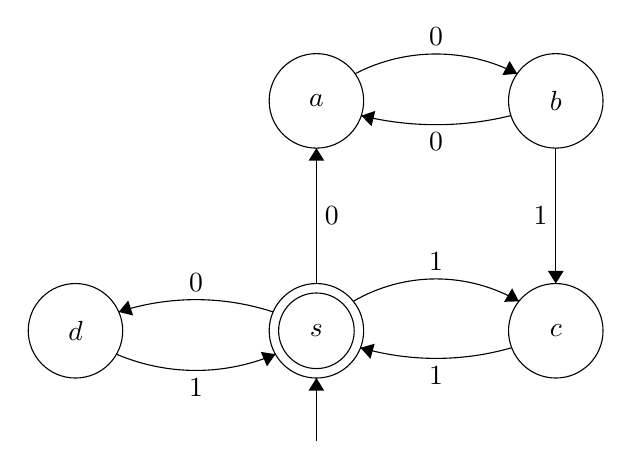
\begin{tikzpicture}[scale=0.2]
			\tikzstyle{every node}+=[inner sep=0pt]
			\draw [black] (22.3,-24.6) circle (3);
			\draw (22.3,-24.6) node {$s$};
			\draw [black] (22.3,-24.6) circle (2.4);
			\draw [black] (22.3,-10) circle (3);
			\draw (22.3,-10) node {$a$};
			\draw [black] (37.5,-10) circle (3);
			\draw (37.5,-10) node {$b$};
			\draw [black] (37.5,-24.6) circle (3);
			\draw (37.5,-24.6) node {$c$};
			\draw [black] (7,-24.6) circle (3);
			\draw (7,-24.6) node {$d$};
			\draw [black] (22.3,-31.6) -- (22.3,-27.6);
			\fill [black] (22.3,-27.6) -- (21.8,-28.4) -- (22.8,-28.4);
			\draw [black] (22.3,-21.6) -- (22.3,-13);
			\fill [black] (22.3,-13) -- (21.8,-13.8) -- (22.8,-13.8);
			\draw (22.8,-17.3) node [right] {$0$};
			\draw [black] (24.747,-8.28) arc (117.4169:62.5831:11.191);
			\fill [black] (35.05,-8.28) -- (34.57,-7.47) -- (34.11,-8.36);
			\draw (29.9,-6.52) node [above] {$0$};
			\draw [black] (34.653,-10.936) arc (-76.14141:-103.85859:19.842);
			\fill [black] (25.15,-10.94) -- (25.8,-11.61) -- (26.04,-10.64);
			\draw (29.9,-12.01) node [below] {$0$};
			\draw [black] (37.5,-13) -- (37.5,-21.6);
			\fill [black] (37.5,-21.6) -- (38,-20.8) -- (37,-20.8);
			\draw (37,-17.3) node [left] {$1$};
			\draw [black] (34.703,-25.675) arc (-73.92814:-106.07186:17.35);
			\fill [black] (25.1,-25.68) -- (25.73,-26.38) -- (26,-25.42);
			\draw (29.9,-26.85) node [below] {$1$};
			\draw [black] (9.746,-23.403) arc (108.10105:71.89895:15.784);
			\fill [black] (9.75,-23.4) -- (10.66,-23.63) -- (10.35,-22.68);
			\draw (14.65,-22.12) node [above] {$0$};
			\draw [black] (19.702,-26.086) arc (-66.90784:-113.09216:12.88);
			\fill [black] (19.7,-26.09) -- (18.77,-25.94) -- (19.16,-26.86);
			\draw (14.65,-27.62) node [below] {$1$};
			\draw [black] (24.636,-22.734) arc (120.35966:59.64034:10.415);
			\fill [black] (35.16,-22.73) -- (34.73,-21.9) -- (34.22,-22.76);
			\draw (29.9,-20.81) node [above] {$1$};
			\end{tikzpicture}
		\end{center}
	
	\item $ (ab+\varepsilon)(b+\varepsilon)^*=(ab+\varepsilon)(b^*+\varepsilon)=abb^*+b^*+ab+\varepsilon=abb^*+b^*+\varepsilon$\\
	Any string starting with an $ a $ followed by one or more $ b $'s, or any string comprised any number of $ b $'s.
	\begin{center}
		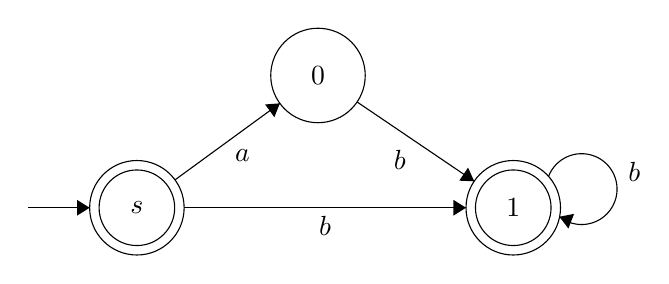
\begin{tikzpicture}[scale=0.2]
		\tikzstyle{every node}+=[inner sep=0pt]
		\draw [black] (17.5,-26.5) circle (2.4);
		\draw [black] (17.5,-26.5) circle (3);
		\draw (17.5,-26.5) node {$s$};
		\draw [black] (29,-18.1) circle (3);
		\draw (29,-18.1) node {$0$};
		\draw [black] (41.4,-26.5) circle (2.4);
		\draw [black] (41.4,-26.5) circle (3);
		\draw (41.4,-26.5) node {$1$};
		\draw [black] (43.637,-24.519) arc (159.25512:-128.74488:2.25);
		\draw (48.68,-24.2) node [right] {$b$};
		\fill [black] (44.33,-27.07) -- (44.9,-27.82) -- (45.26,-26.89);
		\draw [black] (10.6,-26.5) -- (14.5,-26.5);
		\fill [black] (14.5,-26.5) -- (13.7,-26) -- (13.7,-27);
		\draw [black] (19.92,-24.73) -- (26.58,-19.87);
		\fill [black] (26.58,-19.87) -- (25.64,-19.94) -- (26.23,-20.75);
		\draw (24.2,-22.8) node [below] {$a$};
		\draw [black] (31.48,-19.78) -- (38.92,-24.82);
		\fill [black] (38.92,-24.82) -- (38.53,-23.95) -- (37.97,-24.78);
		\draw (34.2,-22.8) node [below] {$b$};
		\draw [black] (20.5,-26.5) -- (38.4,-26.5);
		\fill [black] (38.4,-26.5) -- (37.6,-26) -- (37.6,-27);
		\draw (29.45,-27) node [below] {$b$};
		\end{tikzpicture}
	\end{center}

	\end{enumerate}
\end{document}